\chapter{Machine Learning Algorithms for Food Image Classification}
\lhead{\emph{Machine Learning Algorithms for Food Image Classification}}
This chapter describes actions taken to implement food image classifiers. Each algorithm is firstly briefly introduced, then the details of how was implemented are provided, and finally, the results of image classification are shown.

\section{K-Nearest Neighbours Classifier}

\subsection{Introduction to K-Nearest Neighbours Algorithm}
K-nearest neighbours classifier is one of the simplest machine learning algorithms. To train the classifier, all that needs to be done is saving the training data samples to a computer memory. When deciding a class for a data sample with an unknown class, the classifier calculates the distance between the data sample and every other sample in the data set. Then, the classifier picks the class of the sample according to class labels of k other samples that are located closest to it. Illustration of k-nearest neighbours algorithm performing a classification on a data entity with an unknown class is shown in \autoref{fig:knn}. The rationale behind such a method is based on the assumption that the features that are used to describe the domain points are relevant to their labels in a way that makes close-by points likely to have the same label (Shalev-Shwartz \& Ben-David, 2014). 


\begin{figure}[h]
\centering
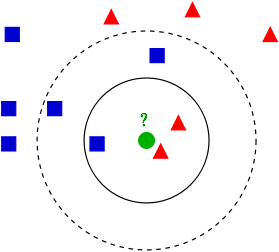
\includegraphics[width=0.3\textwidth]{Figures/knn.png}
\caption{Example of k-NN classification. }
The test sample (green circle) should be classified either to the first class of blue squares or the second class of red triangles. If k = 3 (solid line circle) it is assigned to the second class because there are two triangles and only 1 square inside the inner circle. If k = 5 (dashed line circle) it is assigned to the first class (3 squares vs. two triangles inside the outer circle) \citep{wikipedia_2017}.
\label{fig:knn}
\end{figure}


\subsection{Implementation of a K-Nearest Neighbours Classifier}
 A K-nearest neighbours classifier was imported from the Sckit-learn package. The KNN classifier provided in this package provides many different parameters for modifying the algorithm.  It was decided to try to run classification with images resized to 50x50 pixels. The images also needed to be flattened. Flattening is a process of converting a multidimensional matrix into a vector. To flatten all pictures in the dataset, the height, weight and colour channels of images, were merged into one channel.

 To later test the classification performance, the dataset needed to be split into the separate training and testing datasets. The training dataset, as the name suggests, is used for an algorithm to learn the model and the test dataset is used only for evaluating the performance of the model. At first, it was decided, to use 70 percent of the randomly shuffled dataset as the training data and 30 percent as the test dataset (3168 training samples and 1359 test samples). That means that there were around 790 pictures for each of the four classes. After training a classifier, it was noticed that it performed rather poorly. Therefore it was decided to increase the number of images in the training dataset to 90 percent of the dataset. In this case, there were 4698 examples of training images and 522 examples of testing pictures.
 
It was tried to experiment with what K number of neighbours the classifier worked best, in order to improve the classification accuracy. After running the algorithm multiple times with different values of K, it was observed that the highest classification score was achieved with a K value = 18. However, the best accuracy score which was 36.28 percent was not an acceptable result, and it was necessary to improve the classifier.

 Images in the dataset were resized to the increased 100x100 pixels resolution, in order to test if larger image sizes would help the KNN classifier to perform better. When tested on k= 18 neighbours, the classifier showed the improved accuracy to 45.59 percent. To get a better understanding about how did the classifier perform a confusion matrix was plotted. From the confusion matrix \autoref{fig:k18}, it can be seen that Vanilla ice cream was classified correctly most often from the four classes. The accuracy of predicting it was 78.4 percent. The worst classified class was a salad which achieved only 0.02 percent accuracy.


\begin{figure}[h]
\centering
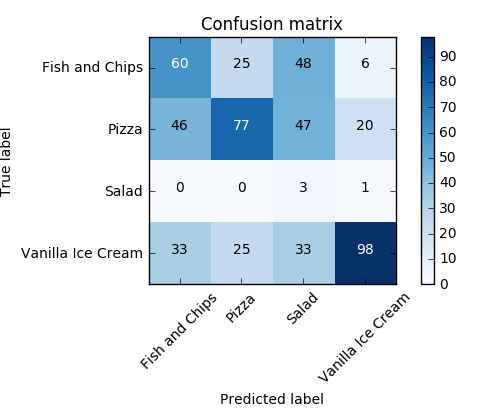
\includegraphics[width=0.5\textwidth]{Figures/conf_k-18.PNG}
\caption{Confusion Matrix of KNN Classifier with K = 18}
\label{fig:k18}
\end{figure}




\subsection{Tuning of Hyperparameters}
Hyperparameters of a machine learning algorithm is a set of parameters that algorithm uses and that have to be specified while training the algorithm e.g.: K- amount of neighbours considered in the KNN classifier. Traditionally, hyperparameters were determined by humans, but the development of computing technology currently allows the use of various search techniques for better parameter optimisation.

There are two methods available for finding the best hyperparameters in the Sckit-learn package. These are an exhaustive grid search - GridSearchCV and a randomised grid search - RandomizedSearchCV.  The Exhaustive grid search tries to run an algorithm with all combinations of hyperparameters provided. The advantage of this approach is that the algorithm will always find the best combination of hyperparameters. However, exhaustive search algorithm has tried every single combination of hyperparameters before choosing the best set. It can be very computationally expensive and take a long time. Randomised search is usually able to find the set of parameters that can perform roughly equivalent than a grid search. The fact that that randomised optimisation could be a better optimisation technique was proven by Bergstra and Bengio who empirically and theoretically demonstrated that randomly chosen trials could be more efficient for hyper-parameter optimisation than trials on a grid \cite{bergstra2012random}.

 It was decided to optimise the following hyperparameters in the  K-nearest neighbours classifier: an amount of neighbours, a weight function that is used, and a distance function used. The number of neighbours considered was from k=1 to k=30. Weight function was either uniform meaning that during the classification the influence of all k neighbours is the same, or distance based, meaning that closer neighbours are more influential when the class of the target image is picked.  For the distance function, Manhattan and Euclidean distance were considered.


It was decided to try running the exhaustive grid search first to get the set of hyperparameters that works best for the classifier.Because hyperparameters sets are independent of each other, it was possible to run hyperparameter optimisation task in a parallel, using multiple cores of a CPU. Still, it took 30 minutes to run the exhaustive search on selected hyperparameters. It was found that the algorithm was most accurate with k = 8 neighbours, the Euclidean distance function, and uniform weights. Then, the algorithm was tested on the test dataset and classified it with 56.32 percent accuracy. More than 10 percent increase in accuracy was a considerable improvement from the previously achieved score.

From a plotted confusion matrix (\autoref{fig:k8}) it can be seen that the optimised KNN classifier was able to predict both pizza and ice cream classes very accurately. This fact is also confirmed in a precision, recall and f score table \autoref{table:1}. An average precision score of these two categories was around 0.8. However, the recall was lower - 0.53. The recall value was smallbecause the classifier misclassified a lot of images from different classes as pizza and vanilla ice cream.



\begin{figure}[h]
\centering
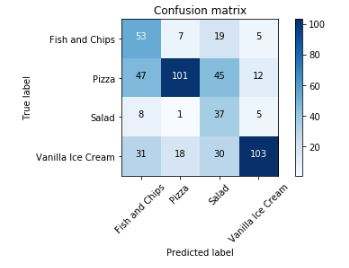
\includegraphics[width=0.6\textwidth]{Figures/knn.JPG}
\caption{Confusion Matrix of KNN classifier with K= 8, Euclidean Distance and Uniform Weights}
\label{fig:k8}
\end{figure}

\begin{table}[h!]
\begin{center}
\begin{tabular}{ |c|c|c|c| } 
 \hline
 Class & precision &   recall & f1-score  \\ \hline
 Fish and Chips    &   0.38   &   0.63  &    0.48   \\
            Pizza   &    0.80  &    0.49 &     0.61 \\
            Salad    &   0.28  &    0.73  &    0.41  \\
Vanilla Ice Cream     &  0.82  &    0.57   &   0.67   \\ \hline
     Average     &  0.69   &   0.56    &  0.59  \\
 \hline
\end{tabular}
\caption{Precision, Recall and F Scores of the best K-NN Classifier}
\label{table:1}
\end{center}
\end{table}


   

\subsection{Results}

To conclude, with right optimisation of hyperparameters K- nearest neighbours classifier can classify images quite accurately. Pictures of a pizza and a vanilla ice cream class were classified much better compared to the images of the other two classes. The most misclassified class was a salad. The reason for that was the fact that there were images of various kinds of salad in the dataset. Because of that variance, salad class images were very scattered in the prediction space, and the classifier was unable to find the right neighbours.

The advantage of the classifier it that it can be trained in a very short time. However, it is was very slow when predicting the class of an unseen image. Because of that, different classification algorithms needed to be tried.
\iffalse
\section{Linear Classification}

Mapping image pixels to functions. 
F(x,W ) = W*x +b
Classifier can find which parts of the image is important for class of the image and which can be ignored (by setting some weights to low values and other to large)
If the dataset is unbalanced the bias for most likely class could be trained as higher than other

\section{Decision Trees}

\fi

\section{Support Vector Machine}

\subsection{Introduction to Support Vector Machine}

Support vector machine is one of the most influential machine learning algorithms \cite{boser1992training}. The algorithm searches for separators between classes that maximises the distance between them. Advantages of this classifier are that it can work very well on high dimensional data. Support vector machine tries to find a separating hyperplane for each class such that distances between separators and each class are as large as possible. A figure showing how a support vector machine chooses a hyperplane for separating two classes can be seen in \autoref{fig:svm}. Because this algorithm works well for a high dimensional data, it was decided to implement a classifier using SVM algorithm.

\begin{figure}[h]
\centering
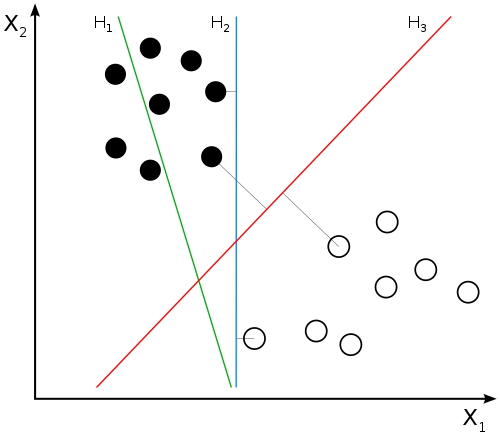
\includegraphics[width=0.5\textwidth]{Figures/svm.PNG}
\caption{Three hyperplanes  that could be used to split the data  }
H3 is selected as a separator because it separates the classes with a largest distance between classes.
\citep{wikipedia_svm}
\label{fig:svm}
\end{figure}


\subsection{Implementation of a SVM Classifier}

Support vector machine module was imported from the Sckit-learn package to start experimenting with it. To understand how the classifier works it was attempted to run the algorithm on our food data set resized to 100 x 100 pixels. At first, it was decided to try to run it with a default set of hyperparameters.

The training of the SVM classifier took around 60 minutes. When it was tested on test image data set, the accuracy achieved was only 25 percent.A confusion matrix was plotted \autoref{fig:svd},  to get a better understanding why the accuracy score was so low. The confusion matrix showed that for some reason the classifier classified all the test dataset as a salad. The hypothesis why the support vector machine classified all the data into the one class was that a decision surface that it learnt was too smooth.

The complexity of decision surface of SVM classifier is controlled by a  hyperparameter C and gamma. C parameter describes by how much the classifier should avoid misclassifying the training data. A little C makes the decision surface smooth but misclassifies more training data, while a high C aims at classifying all training examples correctly. \citep{hyper}. The Gamma parameter defines the influence that a single entity has on the decision boundary.  It was decided, to test what set of C and gamma could help to improve the classification accuracy.



\begin{figure}[h]
\centering
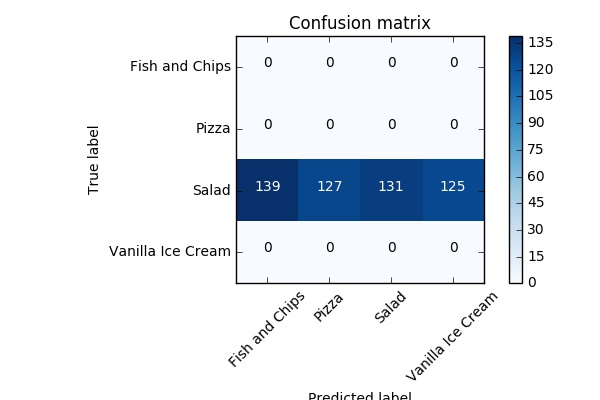
\includegraphics[width=0.5\textwidth]{Figures/svm_default.jpg}
\caption{Confusion Matrix of Support Vector Machine Classifier Trained with Default Parameters}
\label{fig:svd}
\end{figure}


\subsection{Tuning of SVM Hyperparameters}

Because previous SVM model took a long time to train, it was decided to use only 10 percent of the training dataset to find best hyperparameters for this algorithm.

Firstly, it was chosen to increase the value of C. It was increased to the value of 10. With C=10 the algorithm trained on 10 percent of the dataset classified 26 percent of the test data correctly. After plotting the confusion matrix, it was observed that now the classifier predicted all classes \autoref{fig:svm_10_10} but it was very inaccurate in predicting.The C was increased to 100, but that did not improve the classifier.

Finally, the best set of C and gamma hyperparameters was found with randomised grid search. C values of  \(10, 100, 1000, 5000, 10000\) and gamma values  of \(0.0001, 0.0005, 0.001, 0.005, 0.01, 0.1\) were tried. Grid search found that C=10 and gamma = 0.0001 were the best set of parameters. It was reasonable that classifier worked best with the lowest value of gamma because images of food vary a lot and because of that a single image should not have too much influence on the separation lines between classes. It was tried to train the algorithm using a full train data set.

SVM was trained on the whole training dataset with C = 10 and gamma = 0.0001. Despite the fact that the hyperparameters were optimal, the accuracy of the classifier on the training set was only 25 percent. Plotted confusion matrix \autoref{fig:svm2} shown that the model still classified all test dataset as salad class. 

It was deducted that SVM algorithm was unable to classify the dataset correctly because a number of features considered when dividing the hyperplanes was too high. It was decided to use principal component analysis to reduce the number of features and test if that solves the problem.


\begin{figure}[h]
\centering
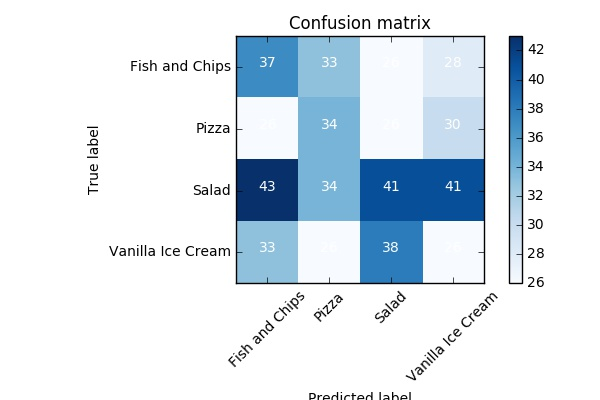
\includegraphics[width=0.5\textwidth]{Figures/svm_10_10.jpg}
\caption{Confusion Matrix of SVM Trained with C= 10}
 \textit{Numbers in squares are: [37 33 26 28],
 [26 34 26 30],
 [43 34 41 41],
 [33 26 38 26]}
\label{fig:svm_10_10}
\end{figure}

\begin{figure}[h]
\centering
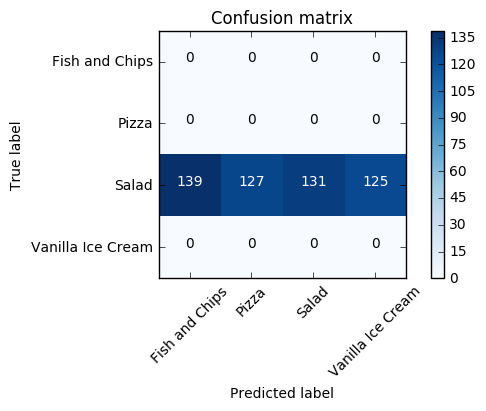
\includegraphics[width=0.5\textwidth]{Figures/svm2.png}
\caption{Confusion Matrix of SVM with C = 10 and Gamma = 0.0001}
\label{fig:svd}
\end{figure}


\subsection{Reduction of  Dimentionality with Principal Component Analysis}
Principal component analysis is a simple, non-parametric method for extracting relevant information from confusing datasets \citep{pca}. It automatically detects strong patterns in the data and ignores the noise. Because food images contain many patterns and are usually noisy, PCA should be a good solution.  

The number of features was reduced from 30000 to 150 using this technique. Then, randomised grid search was performed to find the best C and gamma values for this support vector machine. 
It was found that algorithm classified the training data best with C = 1000 and gamma = 0.0001. After training, it was tried to classify the test dataset. The classifier achieved 60.73 percent accuracy which was the highest score compared to previously tried algorithms. Then a  confusion matrix and a classification report were plotted.From the confusion matrix displayed in \autoref{fig:conf_svm_pca}, it can be seen that all classes except the salad class were correctly predicted around 83 times. The most frequent misclassification was a fish and chips class misclassified as a pizza. From the classification report displayed in    \autoref{table:pca} it can be seen that a vanilla ice cream class had the highest precision and recall. The classifier predicted most of the ice cream pictures correctly. Because of that, it can be concluded that there was a distinct separator between vanilla ice cream class and other classes.

\begin{figure}[h]
\centering
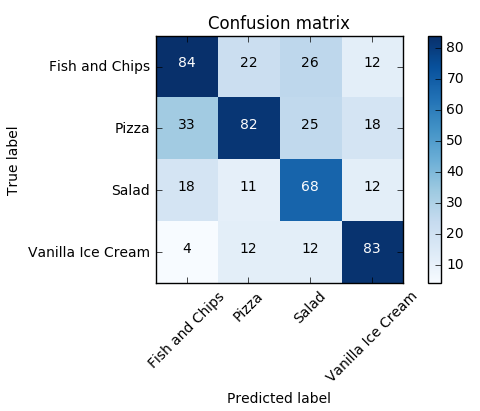
\includegraphics[width=0.5\textwidth]{Figures/conf_svm_pca.PNG}
\caption{Confusion Matrix of SVM Classifier on the Dataset Reduced with PCA}
\label{fig:conf_svm_pca}
\end{figure}

\begin{table}[h!]
\begin{center}
\begin{tabular}{ |c|c|c|c| } 
 \hline
 Class & precision &   recall & f1-score  \\ 
 Fish and Chips    &   0.60    &  0.58    &  0.59 \\
            Pizza   &    0.65   &   0.52   &   0.58 \\
            Salad    &   0.65    &  0.52   &   0.58  \\
Vanilla Ice Cream     &   0.66    &  0.75   &   0.70   \\ \hline
     Average     &  0.61   &   0.61   &   0.61       \\
 \hline
\end{tabular}
\caption{Precision, Recall and F Scores of SVM Model on the Dataset Reduced with PCA }
\label{table:pca}
\end{center}
\end{table}

\section{Summary}

To conclude, the average test accuracy of 60 percent was achieved by both k-nearest neighbours and support vector machine with PCA models. This result proves that machine learning models can be used for classifying the food images. However, 60 percent accuracy is not good enough for using these models for real world applications such as dietary assessment. Therefore, other classification methods need to be explored. In \autoref{sec:intro} it was discussed that since 2012 deep learning has become a dominant method for image classification.  Deep learning methods are going to be presented in the following chapter.